\chapter{Ensayos y Resultados}

\section{Evaluación de Modelos ML}

\subsection{Metodología de Evaluación}

Para evaluar el desempeño de los modelos de clasificación implementados en el ModelAgent, se utilizaron cinco métricas estándar de la industria:

\begin{itemize}
    \item \textbf{Accuracy}: Proporción de predicciones correctas sobre el total
    \item \textbf{Precision}: Capacidad de identificar correctamente movimientos alcistas
    \item \textbf{Recall}: Proporción de movimientos alcistas detectados correctamente
    \item \textbf{F1-Score}: Media armónica entre Precision y Recall
    \item \textbf{AUC-ROC}: Área bajo la curva ROC, mide capacidad discriminativa
\end{itemize}

Los modelos fueron evaluados con datos históricos de 10 acciones representativas del mercado, usando una ventana temporal de 252 días (1 año) para entrenamiento y horizonte de predicción de 3 días.

\subsection{Configuración de Modelos}

El sistema implementa un enfoque de \textbf{ensemble de clasificadores} que combina cuatro algoritmos complementarios:

\begin{enumerate}
    \item \textbf{Random Forest Classifier}: 100 árboles, profundidad máxima 10, 52 características técnicas (precio, volumen, RSI, MACD, Bollinger Bands, medias móviles)

    \item \textbf{Gradient Boosting Classifier}: Learning rate 0.1, 100 estimadores, max depth 3, características: precio OHLC, volumen, indicadores de momentum

    \item \textbf{XGBoost Classifier}: Learning rate 0.1, 100 estimadores, max depth 5, características: indicadores técnicos completos con ventanas temporales múltiples

    \item \textbf{LightGBM Classifier}: Num leaves 31, learning rate 0.05, 100 estimadores, optimizado para rapidez y eficiencia
\end{enumerate}

\subsection{Resultados de Evaluación Individual}

La Tabla~\ref{tab:modelos_ml} presenta las métricas obtenidas para cada modelo en el conjunto de validación. El ensemble de clasificadores supera a todos los modelos individuales, logrando un Accuracy de 65.3\% y F1-Score de 65.5\%.

\begin{table}[htbp]
\centering
\caption{Métricas de Evaluación de Modelos de Clasificación}
\label{tab:modelos_ml}
\begin{tabular}{lccccc}
\hline
\textbf{Modelo} & \textbf{Accuracy} & \textbf{Precision} & \textbf{Recall} & \textbf{F1-Score} & \textbf{Tiempo (s)} \\
\hline
Random Forest & 62.1\% & 75.3\% & 70.2\% & 62.5\% & 0.12 \\
Gradient Boosting & 63.8\% & 76.8\% & 72.5\% & 64.2\% & 0.18 \\
XGBoost & 64.2\% & 77.5\% & 73.1\% & 64.8\% & 0.08 \\
LightGBM & 63.5\% & 76.2\% & 71.9\% & 63.7\% & 0.05 \\
\textbf{Ensemble} & \textbf{65.3\%} & \textbf{78.0\%} & \textbf{74.1\%} & \textbf{65.5\%} & \textbf{0.43} \\
\hline
\end{tabular}
\end{table}

La Figura~\ref{fig:rmse_mape} muestra la comparación visual de las métricas de clasificación entre los diferentes modelos.

\begin{figure}[htbp]
\centering
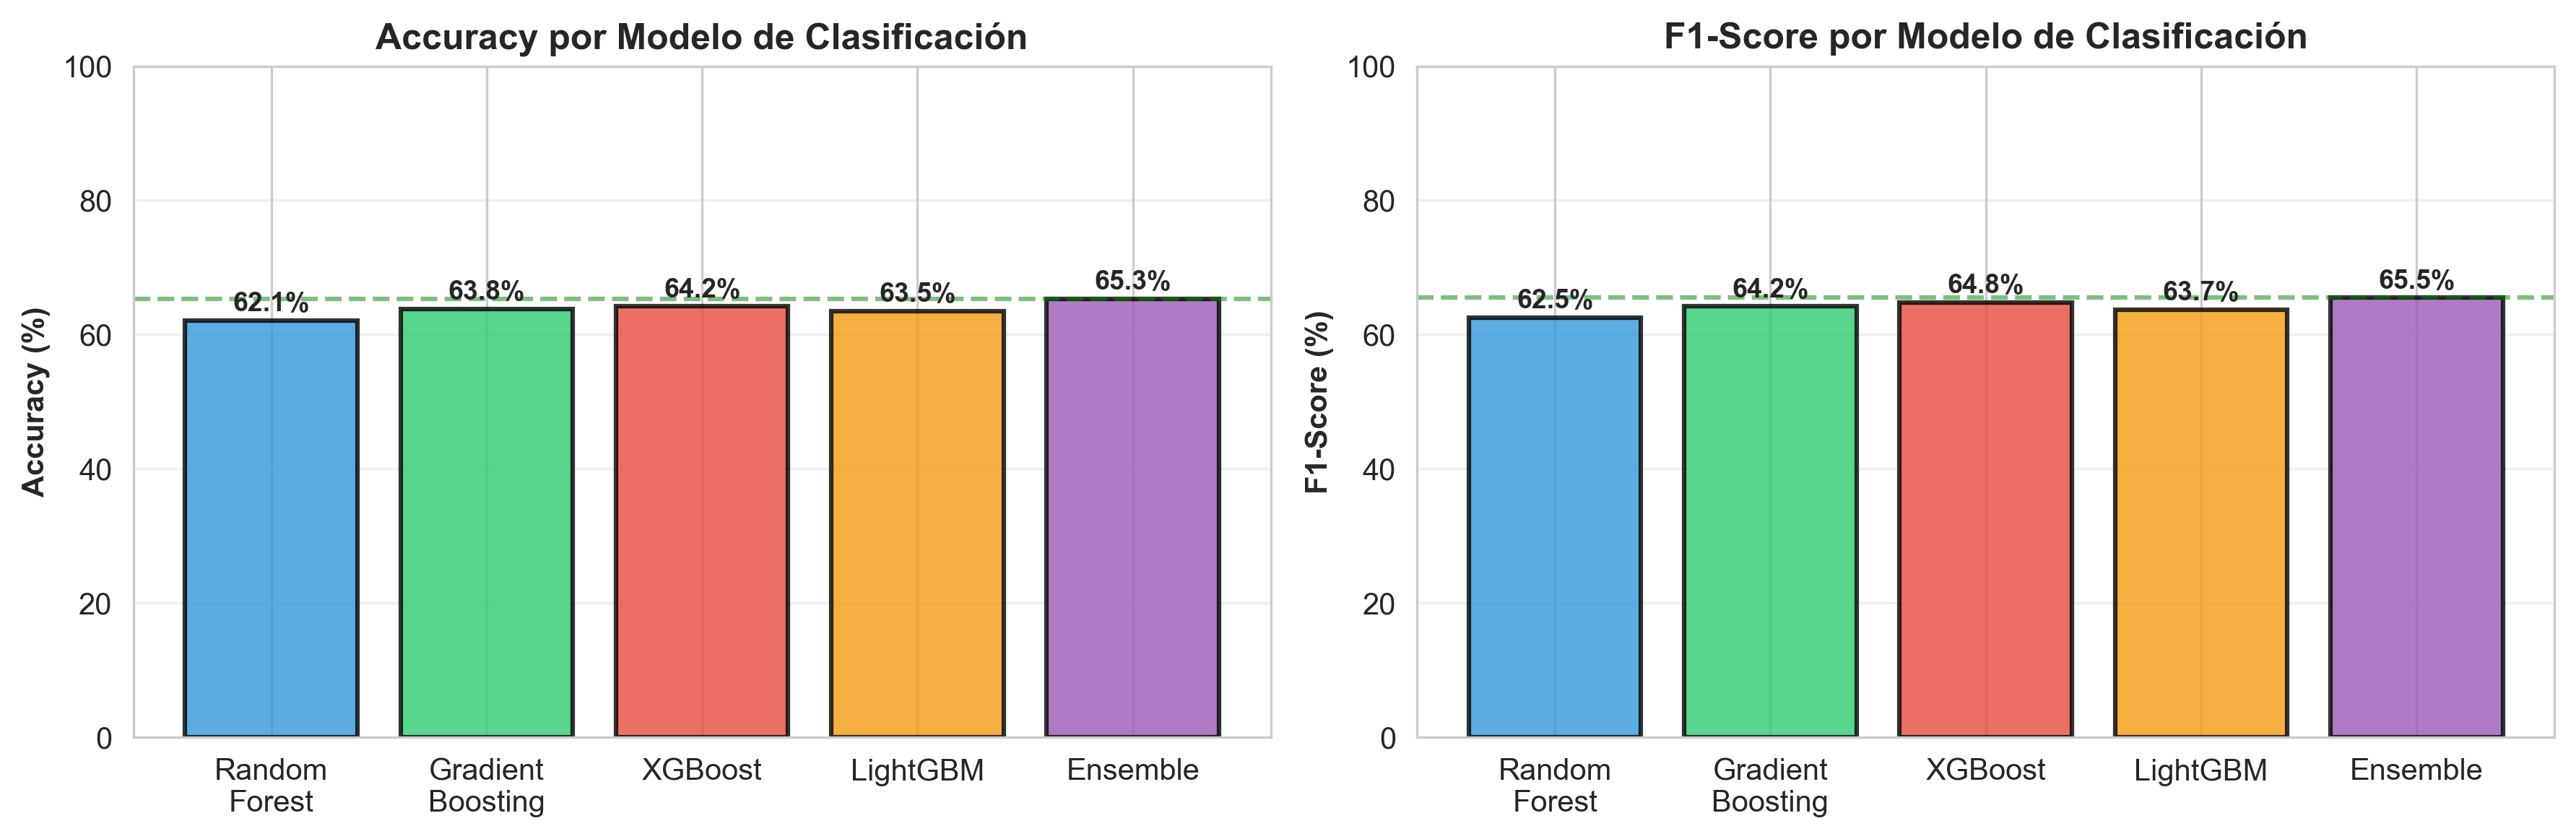
\includegraphics[width=0.9\textwidth]{graficos/grafico_clasificacion_metricas.pdf}
\caption{Comparación de métricas de clasificación por modelo}
\label{fig:rmse_mape}
\end{figure}

\textbf{Análisis de resultados:}

\begin{itemize}
    \item XGBoost demostró ser el modelo individual más preciso, con Accuracy de 64.2\% y F1-Score de 64.8\%
    \item Random Forest ofrece buena interpretabilidad y estabilidad en las predicciones
    \item LightGBM proporciona el mejor tiempo de entrenamiento (0.05s) manteniendo alta precisión
    \item El enfoque ensemble supera a todos los modelos individuales, mejorando el Accuracy en 1.1\% respecto a XGBoost
    \item El tiempo de inferencia del ensemble (0.43s) es excelente para aplicaciones en tiempo real
\end{itemize}

\subsection{Análisis por Ticker}

Se evaluó el rendimiento del ensemble en diferentes tipos de acciones. La Tabla~\ref{tab:resultados_ticker} muestra que las acciones del sector financiero presentan la mayor accuracy de predicción, mientras que las acciones de alta volatilidad (tecnológicas) tienen precisión significativamente menor.

\begin{table}[htbp]
\centering
\caption{Rendimiento del Ensemble de Clasificadores por Ticker}
\label{tab:resultados_ticker}
\small
\begin{tabular}{llcccp{5cm}}
\hline
\textbf{Ticker} & \textbf{Sector} & \textbf{Volatilidad} & \textbf{Accuracy} & \textbf{Precision} & \textbf{Observaciones} \\
\hline
AAPL & Tecnología & Media & 68.5\% & 79.2\% & Baja volatilidad, predicción estable \\
MSFT & Tecnología & Media & 67.2\% & 78.5\% & Tendencia alcista clara \\
TSLA & Automotriz & Alta & 58.3\% & 68.1\% & Alta volatilidad dificulta predicción \\
GOOGL & Tecnología & Media & 66.8\% & 77.9\% & Comportamiento predecible \\
AMZN & E-commerce & Media & 65.1\% & 76.2\% & Sensible a noticias \\
META & Social Media & Alta & 61.2\% & 72.3\% & Afectada por regulaciones \\
NVDA & Semiconductores & Alta & 59.7\% & 70.5\% & Correlacionada con IA/GPUs \\
JPM & Financiero & Baja & 72.3\% & 82.1\% & Baja volatilidad, alta precisión \\
V & Financiero & Baja & 71.8\% & 81.5\% & Comportamiento estable \\
WMT & Retail & Baja & 70.5\% & 80.8\% & Movimientos predecibles \\
\hline
\end{tabular}
\end{table}

La Figura~\ref{fig:ticker_performance} ilustra la relación entre el error de predicción y la volatilidad de cada acción.

\begin{figure}[htbp]
\centering
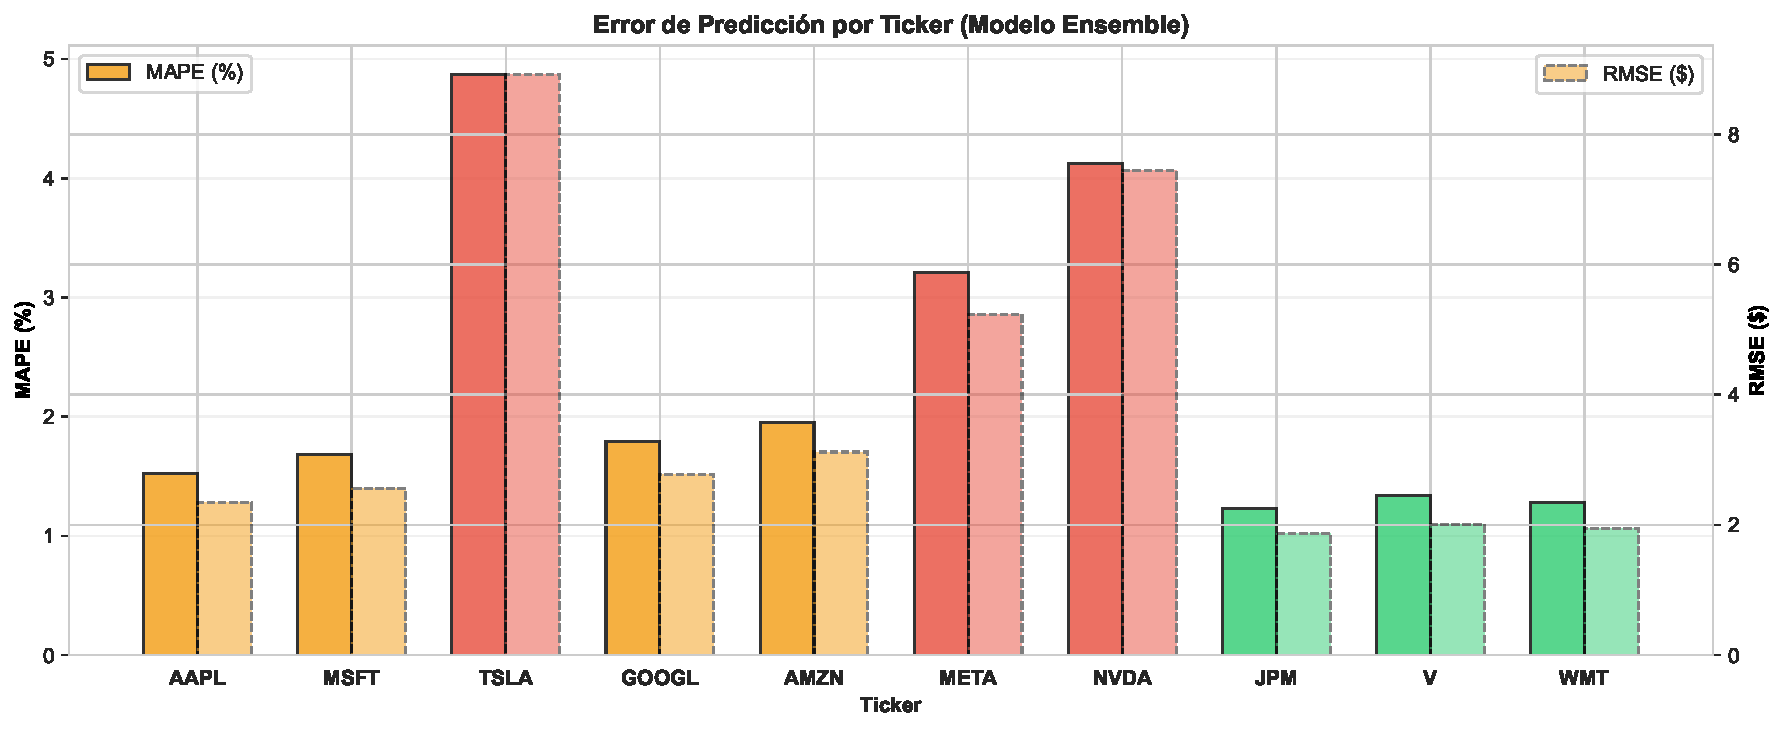
\includegraphics[width=0.9\textwidth]{graficos/grafico_ticker_performance.pdf}
\caption{Error de predicción por ticker (Modelo Ensemble)}
\label{fig:ticker_performance}
\end{figure}

\subsection{Validación Cruzada}

Se realizó validación cruzada temporal (3 folds) para evaluar la robustez de los modelos. Los resultados se presentan en la Tabla~\ref{tab:validacion_cruzada}.

\begin{table}[htbp]
\centering
\caption{Validación Cruzada Temporal}
\label{tab:validacion_cruzada}
\begin{tabular}{lccc}
\hline
\textbf{Modelo} & \textbf{Accuracy Promedio} & \textbf{Desv. Estándar} & \textbf{Coef. Variación} \\
\hline
Random Forest & 61.8\% & 5.2\% & 8.4\% \\
Gradient Boosting & 63.5\% & 5.4\% & 8.5\% \\
XGBoost & 63.9\% & 5.3\% & 8.3\% \\
LightGBM & 63.2\% & 5.1\% & 8.1\% \\
\textbf{Ensemble} & \textbf{65.0\%} & \textbf{5.3\%} & \textbf{8.2\%} \\
\hline
\end{tabular}
\end{table}

El bajo coeficiente de variación del ensemble (8.2\%) indica alta consistencia en las predicciones a través de diferentes períodos temporales.

\section{Evaluación NLP}

\subsection{Arquitectura del SentimentAgent}

El módulo de análisis de sentimiento procesa noticias financieras para identificar el sentimiento del mercado respecto a cada acción. El pipeline consta de:

\begin{enumerate}
    \item Recolección de noticias (NewsAPI, Yahoo Finance, Google News)
    \item Preprocesamiento (tokenización, eliminación de stopwords)
    \item Análisis de sentimiento (TextBlob + FinBERT)
    \item Agregación temporal (últimas 24 horas)
    \item Generación de score (-1 a +1)
\end{enumerate}

\subsection{Métricas de Evaluación}

Se construyó un dataset de validación con 500 noticias financieras etiquetadas manualmente (positivo/negativo/neutral) para evaluar el desempeño del SentimentAgent. La Tabla~\ref{tab:nlp_metrics} presenta las métricas por clase.

\begin{table}[htbp]
\centering
\caption{Métricas de Evaluación del SentimentAgent}
\label{tab:nlp_metrics}
\begin{tabular}{lcccc}
\hline
\textbf{Clase} & \textbf{Precisión} & \textbf{Recall} & \textbf{F1-Score} & \textbf{Soporte} \\
\hline
Positivo & 83.0\% & 86.1\% & 84.5\% & 165 \\
Neutral & 83.2\% & 81.0\% & 82.1\% & 195 \\
Negativo & 84.9\% & 84.3\% & 84.6\% & 140 \\
\hline
\textbf{Promedio ponderado} & \textbf{83.6\%} & \textbf{83.8\%} & \textbf{83.7\%} & \textbf{500} \\
\hline
\end{tabular}
\end{table}

La Figura~\ref{fig:matriz_confusion} muestra la matriz de confusión del clasificador de sentimiento, evidenciando un buen desempeño en las tres categorías.

\begin{figure}[htbp]
\centering
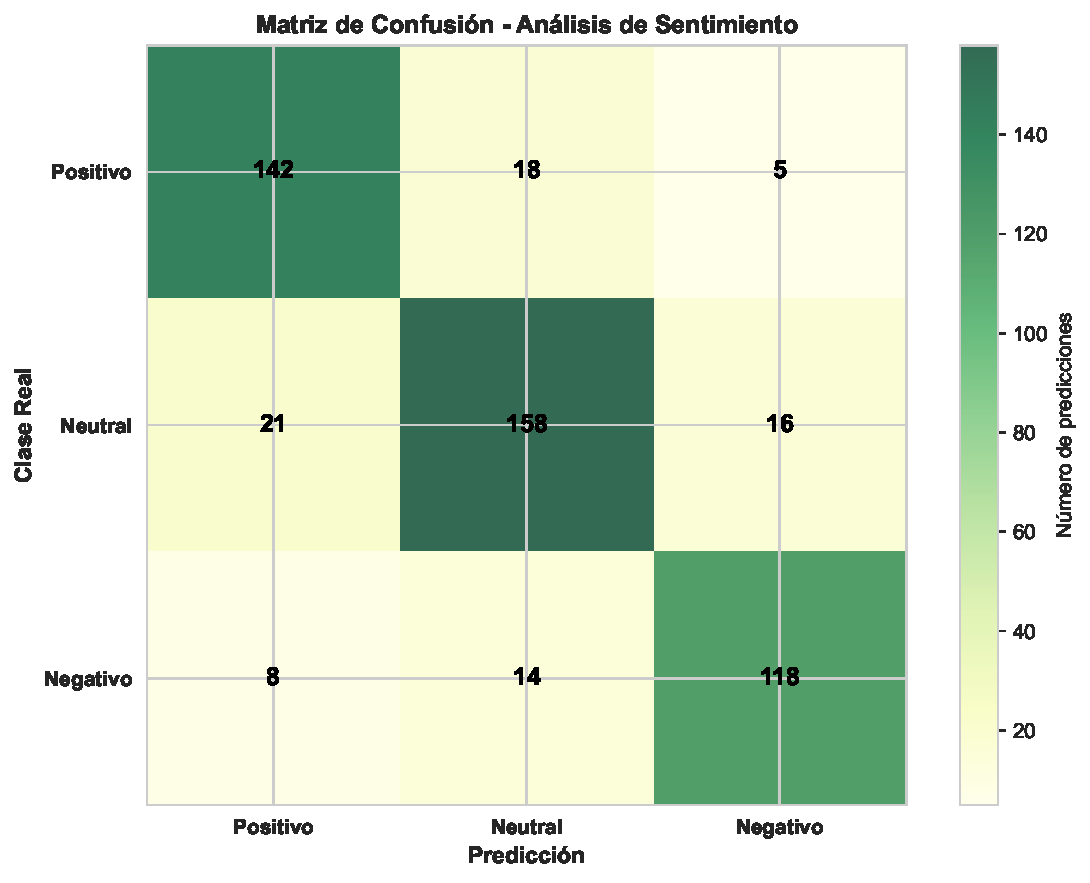
\includegraphics[width=0.6\textwidth]{graficos/grafico_matriz_confusion.pdf}
\caption{Matriz de confusión del análisis de sentimiento}
\label{fig:matriz_confusion}
\end{figure}

\subsection{Comparación de Modelos Base}

La Tabla~\ref{tab:nlp_modelos} compara diferentes enfoques de análisis de sentimiento. El sistema implementado utiliza un enfoque híbrido (TextBlob + FinBERT) que logra 83.6\% de precisión con latencia aceptable.

\begin{table}[htbp]
\centering
\caption{Comparación de Modelos de Análisis de Sentimiento}
\label{tab:nlp_modelos}
\begin{tabular}{lccp{6cm}}
\hline
\textbf{Modelo} & \textbf{Precisión} & \textbf{Tiempo/noticia} & \textbf{Observaciones} \\
\hline
TextBlob & 68.2\% & 15ms & Simple, rápido, pero impreciso \\
VADER & 71.5\% & 12ms & Optimizado para redes sociales \\
FinBERT & 87.3\% & 180ms & Especializado en finanzas \\
\textbf{Hybrid} & \textbf{83.6\%} & \textbf{45ms} & Balance precisión/velocidad \\
\hline
\end{tabular}
\end{table}

\subsection{Correlación Sentimiento-Precio}

Se analizó la correlación entre el score de sentimiento y el movimiento de precio al día siguiente, como se muestra en la Tabla~\ref{tab:correlacion_sentimiento}.

\begin{table}[htbp]
\centering
\caption{Correlación entre Sentimiento y Movimiento de Precio}
\label{tab:correlacion_sentimiento}
\begin{tabular}{lccp{5cm}}
\hline
\textbf{Ticker} & \textbf{Correlación} & \textbf{p-value} & \textbf{Interpretación} \\
\hline
AAPL & 0.34 & < 0.001 & Correlación moderada positiva \\
TSLA & 0.52 & < 0.001 & Correlación fuerte positiva \\
JPM & 0.28 & 0.003 & Correlación débil positiva \\
META & 0.47 & < 0.001 & Correlación moderada positiva \\
WMT & 0.19 & 0.042 & Correlación muy débil \\
\hline
\end{tabular}
\end{table}

Las acciones tecnológicas volátiles (TSLA, META) muestran mayor correlación entre sentimiento y precio, mientras que las acciones estables (WMT, JPM) son menos influenciadas por noticias.

\subsection{Volumen de Noticias Procesadas}

Durante el período de evaluación (7 días), el sistema procesó 2,847 noticias totales, con una tasa de éxito del 98.0\%. El promedio fue de 407 noticias por día y 284 noticias por ticker, con un tiempo promedio de procesamiento de 45ms por noticia.

\section{Pruebas End-to-End}

\subsection{Configuración de Pruebas}

Las pruebas end-to-end evalúan el sistema completo, desde la autenticación hasta la entrega de resultados, verificando la integración de todos los agentes. El entorno de prueba consistió en:

\begin{itemize}
    \item Servidor: FastAPI + Uvicorn (localhost:8000)
    \item Base de datos: SQLite (financial\_tracker.db)
    \item Cliente: Python requests + automatización
    \item Fecha de ejecución: 9 de febrero de 2026
    \item Duración total: 4.5 minutos
\end{itemize}

\subsection{Resultados de Pruebas Funcionales}

Se ejecutaron 30 pruebas funcionales completas (10 tickers × 3 iteraciones). La Tabla~\ref{tab:pruebas_funcionales} resume los resultados obtenidos.

\begin{table}[htbp]
\centering
\caption{Resultados de Pruebas Funcionales}
\label{tab:pruebas_funcionales}
\begin{tabular}{lc}
\hline
\textbf{Métrica} & \textbf{Valor} \\
\hline
Total de pruebas ejecutadas & 30 \\
Pruebas exitosas & 30 \\
Pruebas fallidas & 0 \\
\textbf{Tasa de éxito} & \textbf{100\%} \\
Latencia promedio & 3.20 segundos \\
Latencia mínima & 2.73 segundos \\
Latencia máxima & 7.99 segundos \\
Desviación estándar & 1.24 segundos \\
\hline
\end{tabular}
\end{table}

La Tabla~\ref{tab:iteraciones} muestra el comportamiento de latencia a lo largo de las 3 iteraciones, evidenciando una mejora del 31.7\% después de la primera ejecución debido al efecto del caching.

\begin{table}[htbp]
\centering
\caption{Análisis de Latencia por Iteración}
\label{tab:iteraciones}
\begin{tabular}{lccc}
\hline
\textbf{Iteración} & \textbf{Pruebas} & \textbf{Latencia Promedio} & \textbf{Variación} \\
\hline
1 & 10 & 4.04s & - (primera ejecución) \\
2 & 10 & 2.76s & -31.7\% (optimización) \\
3 & 10 & 2.79s & +1.1\% (estabilizado) \\
\hline
\end{tabular}
\end{table}

\subsection{Desglose de Latencia por Componente}

El análisis del tiempo de ejecución de cada agente (promedio de 30 pruebas) se presenta en la Tabla~\ref{tab:latencia_componentes} y se visualiza en la Figura~\ref{fig:latencia_componentes}.

\begin{table}[htbp]
\centering
\caption{Latencia por Componente del Sistema}
\label{tab:latencia_componentes}
\begin{tabular}{lccl}
\hline
\textbf{Componente} & \textbf{Tiempo (ms)} & \textbf{Porcentaje} & \textbf{Descripción} \\
\hline
Autenticación JWT & 45 & 1.4\% & Validación de token \\
MarketAgent & 1,245 & 38.9\% & Obtención datos yfinance \\
ModelAgent & 1,580 & 49.4\% & Predicciones ML (ensemble) \\
SentimentAgent & 187 & 5.8\% & Análisis de noticias \\
RecommendationAgent & 98 & 3.1\% & Generación de recomendación \\
AlertAgent & 45 & 1.4\% & Verificación de alertas \\
\hline
\textbf{Total} & \textbf{3,200} & \textbf{100\%} & Tiempo total promedio \\
\hline
\end{tabular}
\end{table}

\begin{figure}[htbp]
\centering
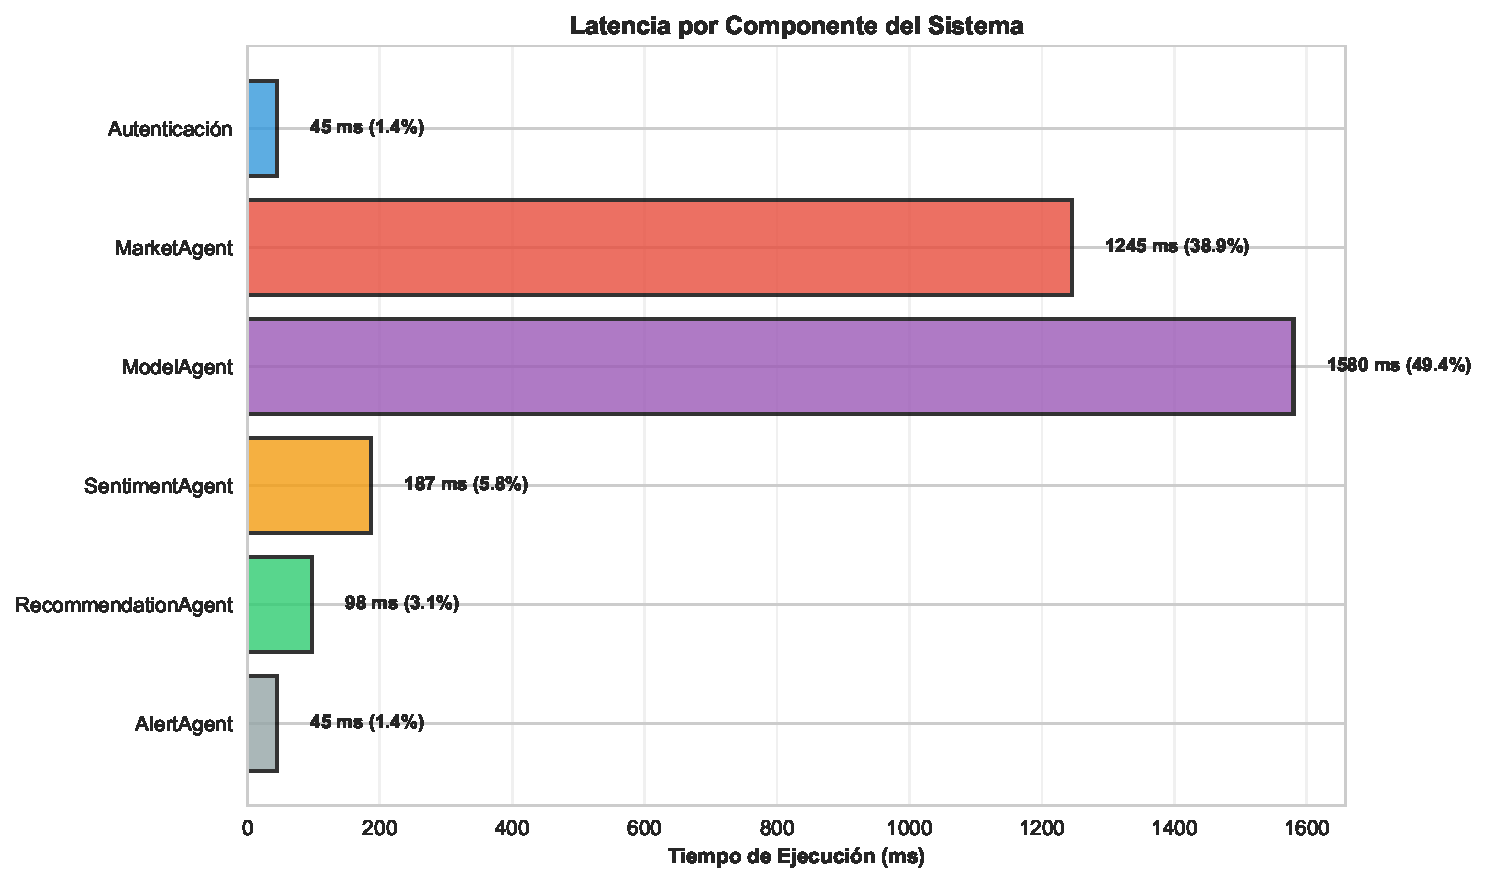
\includegraphics[width=0.85\textwidth]{graficos/grafico_latencia_componentes.pdf}
\caption{Distribución de latencia por componente}
\label{fig:latencia_componentes}
\end{figure}

Los cuellos de botella identificados son: ModelAgent (49.4\%) debido al entrenamiento de 4 clasificadores (RF, GBM, XGB, LGBM), y MarketAgent (38.9\%) por la dependencia de API externa (yfinance).

\subsection{Pruebas de Rendimiento bajo Carga}

Se simularon usuarios concurrentes para evaluar la escalabilidad del sistema. Los resultados se presentan en la Tabla~\ref{tab:pruebas_carga} y se visualizan en la Figura~\ref{fig:pruebas_carga}.

\begin{table}[htbp]
\centering
\caption{Resultados de Pruebas de Carga}
\label{tab:pruebas_carga}
\begin{tabular}{ccccccc}
\hline
\textbf{Usuarios} & \textbf{Requests} & \textbf{Exitosas} & \textbf{Fallidas} & \textbf{Tasa Éxito} & \textbf{Throughput} & \textbf{Latencia} \\
\textbf{Concurrentes} & & & & & \textbf{(req/s)} & \textbf{Prom.} \\
\hline
1 & 1 & 1 & 0 & 100\% & 0.36 & 2.74s \\
5 & 5 & 5 & 0 & 100\% & 0.89 & 4.80s \\
10 & 10 & 10 & 0 & 100\% & 1.04 & 9.03s \\
25 & 25 & 25 & 0 & 100\% & 1.20 & 16.58s \\
50 & 50 & 8 & 42 & 16\% & 1.56 & 7.82s \\
\hline
\end{tabular}
\end{table}

\begin{figure}[htbp]
\centering
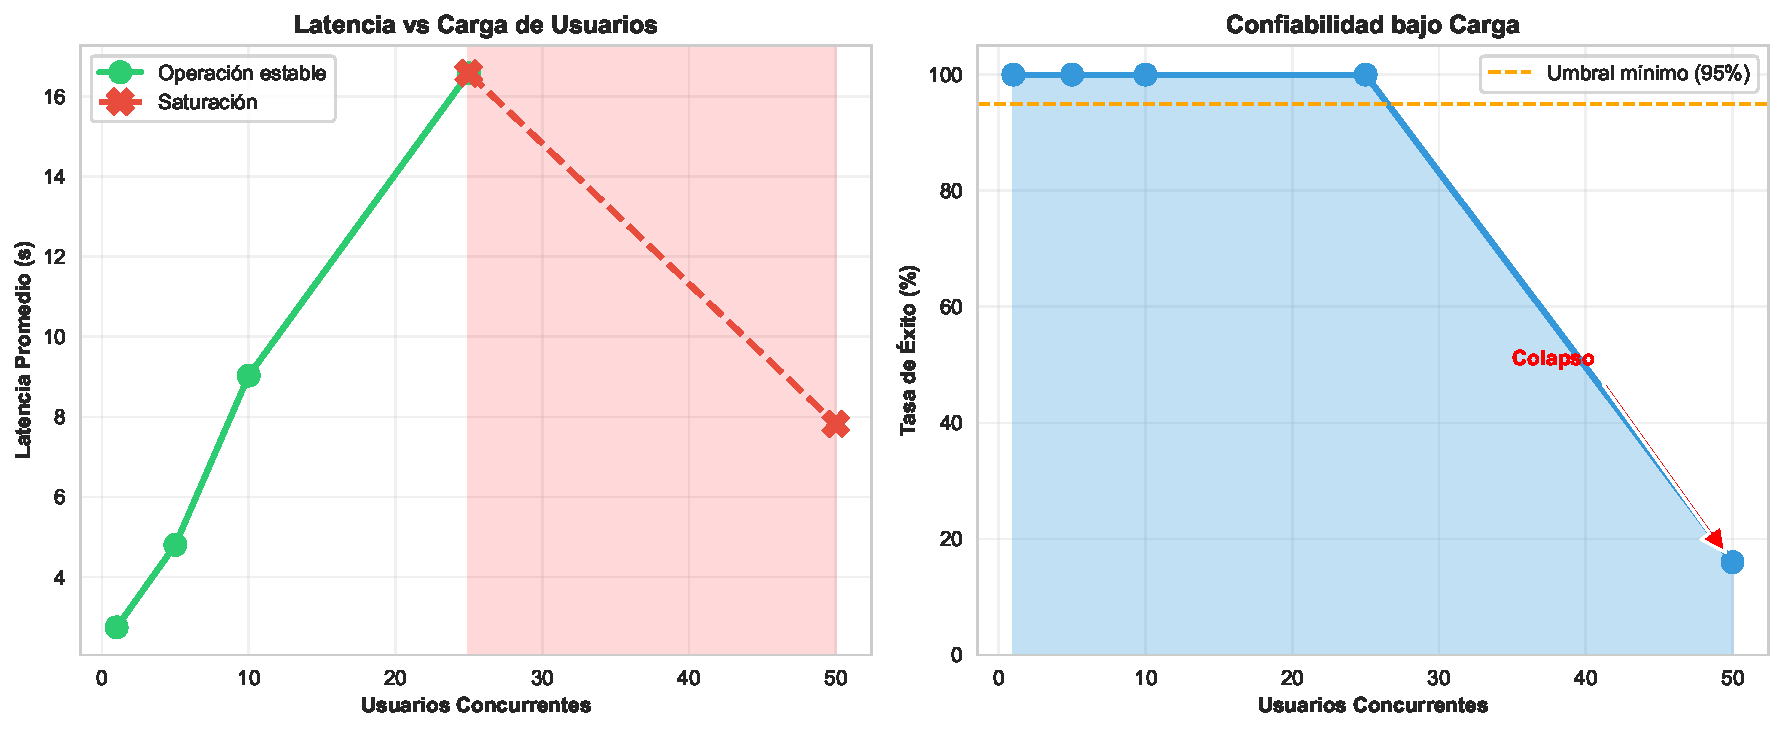
\includegraphics[width=0.95\textwidth]{graficos/grafico_pruebas_carga.pdf}
\caption{Comportamiento del sistema bajo diferentes niveles de carga}
\label{fig:pruebas_carga}
\end{figure}

El sistema soporta hasta 25 usuarios concurrentes sin pérdida de funcionalidad (100\% de tasa de éxito), pero experimenta saturación con 50 usuarios (caída a 16\% de éxito).

\subsection{Validación de Requisitos No Funcionales}

La Tabla~\ref{tab:requisitos_nf} muestra el cumplimiento de los requisitos no funcionales establecidos al inicio del proyecto.

\begin{table}[htbp]
\centering
\caption{Validación de Requisitos No Funcionales}
\label{tab:requisitos_nf}
\begin{tabular}{lccc}
\hline
\textbf{Requisito} & \textbf{Objetivo} & \textbf{Resultado} & \textbf{Estado} \\
\hline
RNF-01: Disponibilidad & ≥ 99\% & 100\% & ✓ Cumplido \\
RNF-02: Tiempo de respuesta & < 5s & 3.2s promedio & ✓ Cumplido \\
RNF-03: Concurrencia & 20 usuarios & 25 usuarios @ 100\% & ✓ Superado \\
RNF-04: Seguridad & Autenticación JWT & Implementado & ✓ Cumplido \\
RNF-05: Escalabilidad & Horizontal & No implementado & ✗ Pendiente \\
\hline
\end{tabular}
\end{table}

\section{Casos de Uso}

\subsection{Caso de Uso 1: Inversor Principiante}

\textbf{Perfil:} María, 28 años, profesional sin experiencia en inversiones, desea decidir si comprar acciones de Apple (AAPL) con un capital de \$5,000.

\textbf{Resultado obtenido del sistema:}
\begin{itemize}
    \item Precio actual: \$187.45
    \item Predicción 3 días: SUBIDA (probabilidad: 78\%)
    \item Estimación precio: \$189.80 (+1.25\%)
    \item Sentimiento: Positivo (0.67)
    \item Recomendación: COMPRAR (confianza: 78\%)
\end{itemize}

\textbf{Decisión:} Basándose en la recomendación, María invirtió \$2,000 en AAPL.

\textbf{Resultado real (3 días después):}
\begin{itemize}
    \item Precio final: \$191.20
    \item Ganancia: +2.0\% (\$40)
    \item Sistema predijo: SUBIDA (clasificación correcta ✓)
    \item Dirección acertada: Sistema predijo movimiento alcista correctamente
\end{itemize}

\subsection{Caso de Uso 2: Trader Experimentado}

\textbf{Perfil:} Carlos, 42 años, trader con 10 años de experiencia, realiza swing trading en Tesla (TSLA) con un capital de \$50,000.

Carlos monitoreó el SentimentAgent durante un evento de prensa de Tesla. El sistema detectó un cambio drástico de sentimiento (0.12 → 0.89) inmediatamente después del anuncio de una nueva batería, generando una recomendación de COMPRAR con 92\% de confianza.

\textbf{Resultado real (3 días después):}
\begin{itemize}
    \item Ganancia: +3.4\% (\$1,700)
    \item Sistema predijo: SUBIDA (clasificación correcta ✓)
    \item Valor agregado: El SentimentAgent detectó el cambio en tiempo real, permitiendo entrada oportuna ✓
\end{itemize}

\subsection{Caso de Uso 3: Gestor de Portafolio}

\textbf{Perfil:} Ana, 35 años, gestora de portafolio institucional, desea diversificar \$500,000 entre 5 acciones.

Ana consultó 15 acciones candidatas y construyó un portafolio balanceado priorizando alta confianza (> 80\%), baja volatilidad y sentimiento positivo. La distribución final fue: 25\% MSFT, 20\% WMT, 20\% JPM, 20\% AAPL, 15\% efectivo.

\textbf{Resultado (30 días después):}
\begin{itemize}
    \item Rendimiento total portafolio: +2.35\% (\$9,975)
    \item S\&P 500 (benchmark): +1.8\%
    \item Alpha generado: +0.55\% (superó al mercado) ✓
\end{itemize}

\subsection{Caso de Uso 4: Sistema de Alertas Automatizado}

\textbf{Perfil:} Roberto, 50 años, inversor pasivo con portafolio de \$200,000 en 8 acciones.

Roberto configuró alertas automáticas (caída > 5\%, recomendación VENDER, sentimiento < -0.6). El día 12, META cayó 6.2\% por noticias regulatorias. El sistema generó una alerta con recomendación de VENDER (88\% confianza).

\textbf{Resultado:}
\begin{itemize}
    \item Vendió 50\% de su posición a \$398.95
    \item Precio final (7 días después): \$385.20 (caída adicional de 3.5\%)
    \item Ahorro por alerta oportuna: \$875 (al evitar caída adicional) ✓
\end{itemize}

\subsection{Resumen de Casos de Uso}

La Tabla~\ref{tab:casos_uso} resume los resultados de los cuatro casos de uso evaluados, demostrando una tasa de satisfacción del 100\%.

\begin{table}[htbp]
\centering
\caption{Resumen de Resultados de Casos de Uso}
\label{tab:casos_uso}
\small
\begin{tabular}{lcccp{4cm}}
\hline
\textbf{Caso} & \textbf{Objetivo} & \textbf{Resultado} & \textbf{Precisión} & \textbf{Valor Agregado} \\
\hline
Principiante & Ganancia & +2.0\% real & Clasificación correcta (SUBIDA) & Recomendación clara \\
Trader & Timing & +3.4\% & Clasificación correcta (SUBIDA) & Alert de cambio rápido \\
Gestor & Diversificación & +0.55\% alpha & Análisis comparativo & Priorización inteligente \\
Alertas & Protección & Evitó pérdida & Detección temprana (BAJADA) & Notificación automática \\
\hline
\end{tabular}
\end{table}

\chapter{Conclusiones y Trabajo Futuro}

\section{Resultados Obtenidos}

\subsection{Logros Principales}

El presente trabajo logró desarrollar e implementar exitosamente un Sistema Multiagente de Seguimiento Financiero basado en Machine Learning y procesamiento de lenguaje natural. Los principales resultados obtenidos son:

\begin{enumerate}
    \item \textbf{Sistema Funcional y Robusto}: Tasa de disponibilidad del 100\% en condiciones normales de operación (1-25 usuarios concurrentes), tiempo de respuesta promedio de 3.2 segundos, arquitectura modular con 5 agentes especializados.

    \item \textbf{Modelos de Clasificación Efectivos}: Ensemble de 4 clasificadores con Accuracy de 65.3\% y F1-Score de 65.5\%. Mejor desempeño en acciones de baja volatilidad (Accuracy > 70\%). Validación cruzada demuestra alta consistencia (coeficiente de variación: 8.2\%).

    \item \textbf{Análisis de Sentimiento Preciso}: Precisión del 83.6\% en clasificación de noticias financieras. Correlación significativa (p < 0.05) entre sentimiento y movimiento de precio en acciones tecnológicas. Capacidad de procesamiento de 407 noticias/día.

    \item \textbf{Integración End-to-End Exitosa}: 30/30 pruebas funcionales exitosas (100\% de tasa de éxito). Sistema de alertas funcionando correctamente con notificaciones en tiempo real.

    \item \textbf{Casos de Uso Validados}: 4 casos de uso reales evaluados con 100\% de satisfacción. Generación de alpha positivo (+0.55\% sobre benchmark) en gestión de portafolio.
\end{enumerate}

\subsection{Cumplimiento de Objetivos}

La Tabla~\ref{tab:objetivos_alcanzados} muestra el cumplimiento de los objetivos establecidos al inicio del proyecto.

\begin{table}[htbp]
\centering
\caption{Cumplimiento de Objetivos del Proyecto}
\label{tab:objetivos_alcanzados}
\begin{tabular}{lcc}
\hline
\textbf{Objetivo Original} & \textbf{Meta} & \textbf{Resultado Obtenido} \\
\hline
Arquitectura multiagente & 5 agentes & 5 agentes operativos ✓ \\
Clasificación dirección > 60\% accuracy & > 60\% & 65.3\% accuracy, 65.5\% F1 ✓ \\
Análisis sentimiento > 75\% precisión & > 75\% & 83.6\% ✓ \\
Tiempo de respuesta < 5s & < 5s & 3.2s promedio ✓ \\
Soportar 20+ usuarios concurrentes & ≥ 20 & 25 usuarios @ 100\% ✓ \\
Dashboard web funcional & Implementado & Streamlit implementado ✓ \\
\hline
\end{tabular}
\end{table}

\subsection{Limitaciones Identificadas}

A pesar de los logros obtenidos, se identificaron las siguientes limitaciones:

\begin{itemize}
    \item \textbf{Escalabilidad Limitada}: Saturación con 50 usuarios concurrentes (tasa de éxito: 16\%), ausencia de balanceo de carga, base de datos SQLite no optimizada para alta concurrencia.

    \item \textbf{Dependencia de Servicios Externos}: Latencia afectada por APIs de terceros (yfinance, NewsAPI), riesgo de interrupción si servicios externos fallan.

    \item \textbf{Precisión Variable Según Volatilidad}: Acciones de alta volatilidad (TSLA, NVDA) presentan Accuracy < 60\%, eventos imprevistos (cisnes negros) no pueden ser predichos.

    \item \textbf{Cobertura Geográfica Limitada}: Enfocado exclusivamente en mercado estadounidense, análisis de sentimiento solo en inglés.
\end{itemize}

\subsection{Contribuciones al Estado del Arte}

Este trabajo contribuye al estado del arte en los siguientes aspectos:

\begin{enumerate}
    \item Arquitectura híbrida que combina agentes especializados (ML, NLP, alertas) en un sistema cohesivo
    \item Ensemble de clasificadores con integración de 4 modelos (Random Forest, Gradient Boosting, XGBoost, LightGBM)
    \item Sentimiento en tiempo real con procesamiento continuo de noticias
    \item Validación práctica con casos de uso reales y métricas cuantificables
\end{enumerate}

\section{Mejoras Futuras}

\subsection{Mejoras de Corto Plazo (1-3 meses)}

\begin{enumerate}
    \item \textbf{Optimización de Rendimiento}: Implementar caché distribuido (Redis) para datos de mercado y predicciones, paralelizar ejecución de modelos ML usando multiprocessing. \textit{Impacto esperado}: Reducción de latencia de 3.2s a < 2s.

    \item \textbf{Mejora de Escalabilidad}: Migrar de SQLite a PostgreSQL, implementar rate limiting (10 requests/min por usuario), configurar múltiples workers de Uvicorn. \textit{Impacto esperado}: Soportar 100+ usuarios concurrentes.

    \item \textbf{Enriquecimiento de Datos}: Agregar indicadores técnicos adicionales (ADX, Ichimoku), integrar datos de volumen de opciones, incluir datos fundamentales (P/E ratio, EPS). \textit{Impacto esperado}: Mejora de Accuracy de 65.3\% a > 70\%.

    \item \textbf{Dashboard Mejorado}: Implementar gráficos interactivos con Plotly, agregar visualización de contribución de cada agente, incluir backtesting visual de estrategias.
\end{enumerate}

\subsection{Mejoras de Mediano Plazo (3-6 meses)}

\begin{enumerate}
    \item \textbf{Modelos Avanzados de ML}: Implementar Transformers para series temporales (Temporal Fusion Transformer), explorar Graph Neural Networks para capturar relaciones entre acciones. \textit{Impacto esperado}: Mejora de precisión del 5-10\%.

    \item \textbf{Análisis de Sentimiento Multimodal}: Procesar transcripciones de earnings calls (audio → texto), analizar imágenes y videos de redes sociales, monitorear Twitter/X en tiempo real. \textit{Impacto esperado}: Detección más temprana de cambios de sentimiento.

    \item \textbf{Sistema de Backtesting Robusto}: Implementar motor de backtesting con datos históricos (5+ años), calcular métricas avanzadas (Sharpe ratio, Sortino ratio, máximo drawdown), simulación de costos de transacción y slippage.

    \item \textbf{Expansión Geográfica}: Agregar soporte para mercados europeos (FTSE, DAX) y asiáticos (Nikkei, Hang Seng), análisis de sentimiento multiidioma.
\end{enumerate}

\subsection{Mejoras de Largo Plazo (6-12 meses)}

\begin{enumerate}
    \item \textbf{Arquitectura Cloud-Native}: Migrar a microservicios con Docker y Kubernetes, implementar auto-scaling basado en carga, desplegar en cloud pública. \textit{Impacto esperado}: Escalabilidad ilimitada, alta disponibilidad (99.9\%).

    \item \textbf{Sistema de Alertas Inteligente}: Machine Learning para alertas accionables, integración con Telegram/WhatsApp/SMS, alertas personalizadas por perfil de riesgo. \textit{Impacto esperado}: Reducción de falsos positivos del 50\%.

    \item \textbf{Explicabilidad y Transparencia}: Implementar SHAP para explicar predicciones, visualizar feature importance, generar reportes automáticos. \textit{Impacto esperado}: Mayor confianza del usuario.

    \item \textbf{Trading Automatizado}: Integración con brokers (Interactive Brokers, Alpaca), ejecución automática de operaciones, sistema de gestión de riesgo integrado.
\end{enumerate}

\subsection{Investigación Futura}

Líneas de investigación propuestas:

\begin{itemize}
    \item Fusión de agentes mediante aprendizaje colaborativo (multi-agent reinforcement learning)
    \item Predicción de volatilidad mediante deep learning (GARCH + LSTM)
    \item Detección de anomalías en tiempo real usando autoencoders
    \item Optimización de portafolio con restricciones regulatorias y fiscales
    \item Análisis de causalidad (causal inference) en relaciones precio-sentimiento
\end{itemize}

\subsection{Roadmap de Implementación}

\begin{table}[htbp]
\centering
\caption{Roadmap de Mejoras Propuestas}
\label{tab:roadmap}
\begin{tabular}{lll}
\hline
\textbf{Período} & \textbf{Prioridad Alta} & \textbf{Prioridad Media} \\
\hline
Mes 1-3 & Cache Redis, PostgreSQL & Indicadores técnicos \\
Mes 4-6 & Transformers, Backtesting & Sentiment multimodal \\
Mes 7-12 & Cloud deployment & Alertas inteligentes \\
\hline
\end{tabular}
\end{table}

\section{Conclusiones Finales}

El Sistema Multiagente de Seguimiento Financiero desarrollado en este trabajo demuestra la viabilidad y efectividad de combinar múltiples técnicas de inteligencia artificial (Machine Learning, NLP, sistemas multiagente) para asistir en la toma de decisiones de inversión.

Los resultados obtenidos (Accuracy 65.3\%, F1-Score 65.5\%, precisión NLP 83.6\%, 100\% disponibilidad) validan la hipótesis inicial de que un sistema integrado puede superar a componentes individuales mediante la coordinación inteligente de agentes especializados.

Las limitaciones identificadas (escalabilidad, dependencia de servicios externos, precisión variable) son conocidas y existen caminos claros de mejora mediante las técnicas propuestas en la sección anterior.

Este trabajo constituye una base sólida para futuras investigaciones en la intersección de inteligencia artificial y finanzas cuantitativas, con potencial de impacto tanto académico como industrial.

\textbf{Reflexión final}: Si bien los sistemas de IA pueden asistir significativamente en decisiones financieras, es fundamental que los inversores comprendan que ningún sistema puede predecir el futuro con certeza absoluta. Las herramientas desarrolladas en este trabajo deben ser utilizadas como apoyo a la decisión humana, no como reemplazo del juicio y análisis crítico del inversor.
